\section{Temario} \label{syllabus}

\begin{figure}[!thpb]
    \centering
    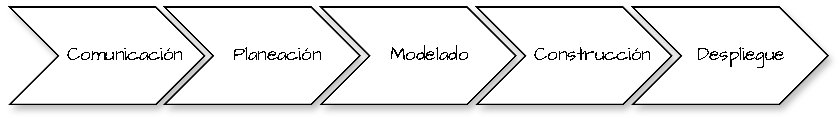
\includegraphics[width=0.7\textwidth]{assets/proceso_pressman_white}
    \caption{Proceso del Software - Pressman}
    \label{fig:proceso_pressman}
\end{figure}

Para el temario del documento final de proyecto se considerará una estructura que describa bien la naturaleza del proyecto y que además se adecúe a este que, después de todo, será un producto de software.

De acuerdo a la ingeniería de software, el software tiene un ciclo de vida o un \say{proceso del software}, el cual se modela de acuerdo a la metodología de desarrollo sobre la cual se realice. Sin embargo, varios autores concuerdan en que existen ciertas etapas estructurales ajenas a cualquier metodología. Según \textit{Pressman} \cite[13]{pressmanSoftwareEngineeringPractitioner2010}, estas etapas serían las indicadas en la figura \ref{fig:proceso_pressman}.

Por su lado, \textit{Sommerville} las simplifica en las 4 etapas mostradas en la figura \ref{fig:proceso_sommerville}.

\begin{figure}[!thpb]
    \centering
    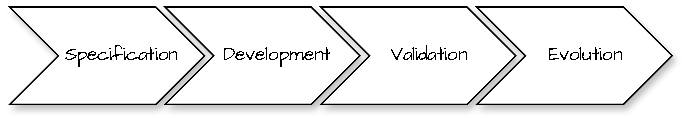
\includegraphics[width=0.7\textwidth]{assets/proceso_sommerville_white.pdf}
    \caption{Proceso del Software - Sommerville}
    \label{fig:proceso_sommerville}
\end{figure}

El temario del documento final del proyecto obedecerá entonces a esta definiciones del proceso de software para no depender estrictamente de la metodología usada.

Nótese, sin embargo, que este temario es tentativo, lo cual quiere decir que pueden surgir cambios durante la realización del proyecto.

\begin{tcolorbox}[breakable]

    \subsection*{\Large{Índice}}
    \begin{syllabus}
        \item[0.] Apartados Preliminares
        \begin{itemize}
            \item Presentación
            \item Agradecimientos
            \item Resumen
            \item Índice
            \item Glosario
        \end{itemize}
    \end{syllabus}

    \begin{syllabus}
        \item \textbf{Generalidades del proyecto:}
        \begin{syllabus}
            \item \textbf{Introducción:} Describirá los antecedentes del proyecto, así como la problemática que se ha identificado, para la cual se plantea una solución a través del objetivo. De igual modo se hará referencia a la justificación del proyecto y los alcances y límites que se plantearon durante su gestación.
            \item \textbf{Marco Referencial:} Se proporciona el contexto general en el cual se sitúa el proyecto. Se describen temas relevantes al tópico principal y que buscan delimitarlo en varios aspectos que pueden ser históricos, geográficos, sociales, políticos, económicos, tecnológicos, etc.
            \item \textbf{Marco Teórico:} Se proporcionan las bases teóricas sobre las cuales se fundamenta el proyecto. se presentarán todos los conceptos, definiciones, técnicas y/o procedimientos que se han de tomar en cuenta para el desarrollo del proyecto y para su correcta comprensión.
        \end{syllabus}
        \item \textbf{Proceso del Software:} Como se explica al inicio de la sección \ref{syllabus}, esta parte del temario reflejará el ciclo de vida común del software. El orden no refleja el orden que se adopte realmente, el cual no será de tipo cascada, sino iterativo, pero como bloques fundamentales del proceso del software, tendrán la información relevante a cada etapa o cada esfuerzo realizado dentro de cada etapa.
        \begin{syllabus}
            \item Especificación de requerimientos de software \cite[104]{pressmanSoftwareEngineeringPractitioner2010}
            \item Modelado y Diseño
            \item Desarrollo y Construcción
            \item Pruebas y Validaciones (Tests)
            \item Despliegue
        \end{syllabus}
        \item \textbf{Integración en el SIAI:} El paquete ya desplegado se integrará en un \textit{fork} del SIAI. En este apartado se hará una bitácora del proceso y se expondrán los resultados del mismo.
        \item \textbf{Resultados y Conclusiones:} El resultado general del proyecto y algunas recomendaciones para seguir trabajando en él, siendo especialmente importante considerando la naturaleza \textit{open source} y colaborativa del paquete a desarrollar. Se deben dar algunas ideas para seguir desarrollando las siguientes versiones del software.
    \end{syllabus}

    \begin{itemize}
        \item Bibliografía y Referencias
        \item Anexos
    \end{itemize}
\end{tcolorbox}